% !TEX root = ../main.tex


\section{Description of Sample Application}

To illustrate the development and analysis process of a design using the previously described 
statechart semantics, we will discuss a quadrotor helicopter or quadrotor application similar to 
the one presented by Syriani et al.~\cite{Syriani_2019}.

The application will focus on the incremental design of some of the functionality required by drone model.
The structure of the model at each abstraction level restrict farther development of the model to 
refinements that obey the rules in Event-B. This will allow us to prove properties of the model a 
very strategic fashion as properties proven of early abstraction levels are preserve in later refinements.

The first abstraction of the model will shown in figure~\ref{fig:drone}
\begin{figure}[!h]
	\vspace{-.4cm}
	\centering
	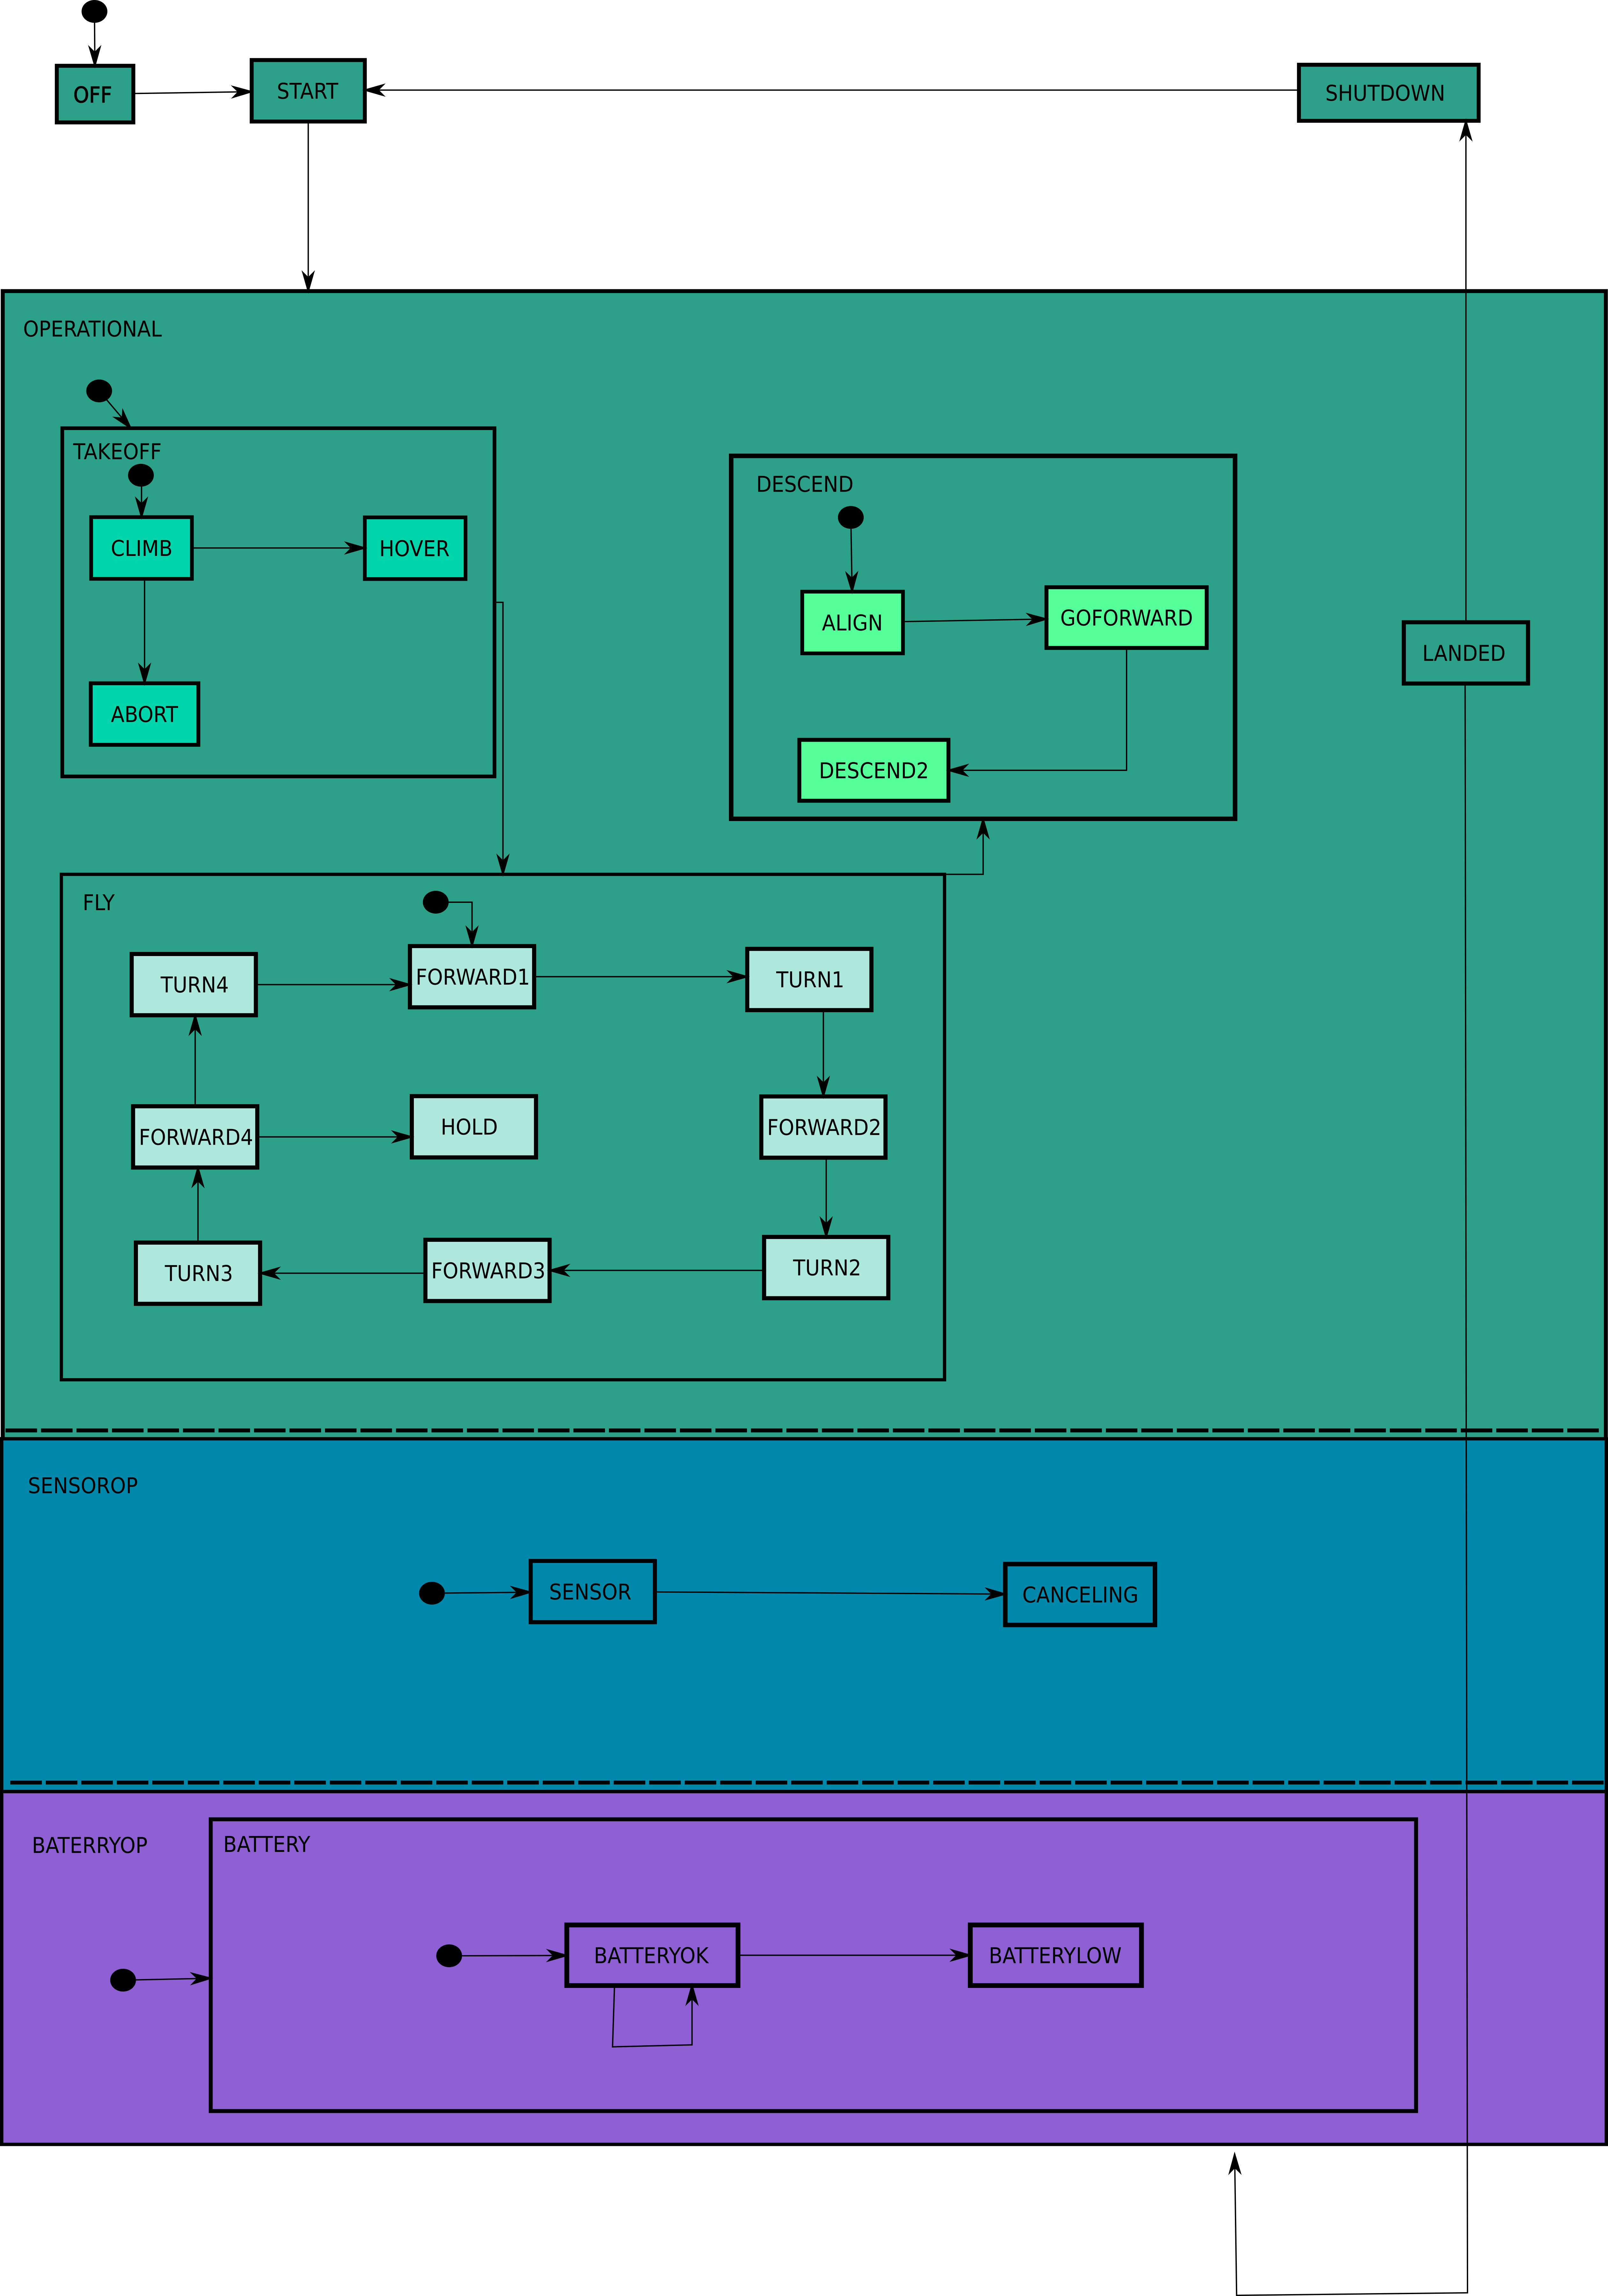
\includegraphics[width=0.99\textwidth]{figures/drone.png}
	\caption{Statechart of drone application. 1. Abstract level including only generic behavior 
	2. Refinement level introducing details for TakeOff 3. Refinement level for descending capabilities 
	4. Refinement level for battery consumption functionality. NOTE: this figure still needs a lot of work}
	\label{fig:drone}
	\vspace{-.4cm}
\end{figure} 
% \emph{Describe the Drone case study including refinements and things we would verify}
